\section*{Arithmetics in Paging (Size, Page Numbers, PTE numbers)}
\begin{minipage}{0.55\linewidth}
  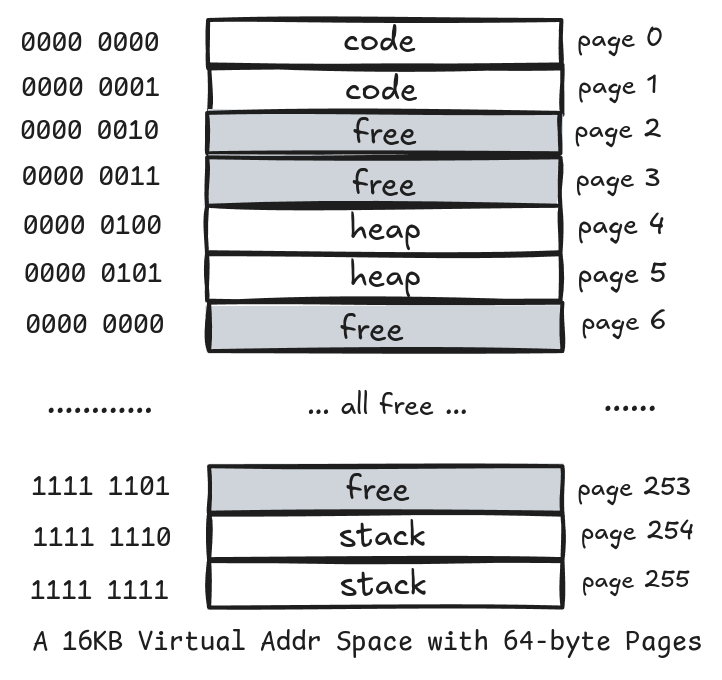
\includegraphics[width=\linewidth]{imgs/virtual_addr_eg}
  \flushleft
  \begin{itemize}
  \item $S_{\text{AS}}$ = 16KB = $16 \times 1024 = 2^{4} \times 2^{10} = 2 ^{14}$B
  \item V Addr bit width = $\log_2 S_{\text{AP}} = 14$
  \item $S_{\text{P}}$ = 64B = $2^{6}$B
  \item \textbf{Offset} bit width = $\log_2 S_{\text{P}} = 6$
  \item VPN bit width = 14 - 6 = 8
  \item $N_{\text{P}}$ = $\frac{S_{\text{AS}}}{S_{\text{P}}} = \frac{2^{14}}{2^{6}} = 2^{8}$
  \item $N_{\text{PTE}} = N_{\text{P}} = 2^{8} = 256$ (linear PT)
  \end{itemize}
\end{minipage}
\begin{minipage}{0.45\linewidth}
  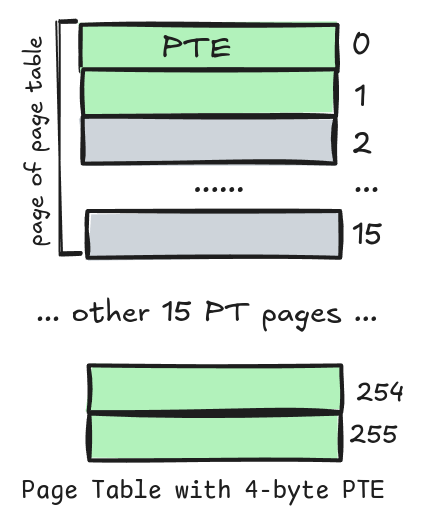
\includegraphics[width=\linewidth]{imgs/pte_4byte}
  \flushleft
  \begin{itemize}
  \item $S_{\text{PTE}} =4$B
  \item $S_{\text{PT}} = N_{\text{PTE}} \times S_{\text{PTE}} = 1\text{KB} $
  \item Page table can be divided into pages (for 2-level PT)
  \item[] $S_{\text{PTP}} = \frac{S_{\text{PT}}}{S_{\text{P}}} = \frac{1024}{64} = 16$
  \item Each PDE points to a PTP of 16 PTEs
  \end{itemize}
\end{minipage}
